\section{Resultados de las simulaciones}
Muchas modelos han sido generados, y muchas simulaciones han sido creadas para el estudio del comportamiento de la epidemia del COVID-19. En Chile, en particular, hay estudios hechos por diversas universidades e investigadores.

\begin{figure}
    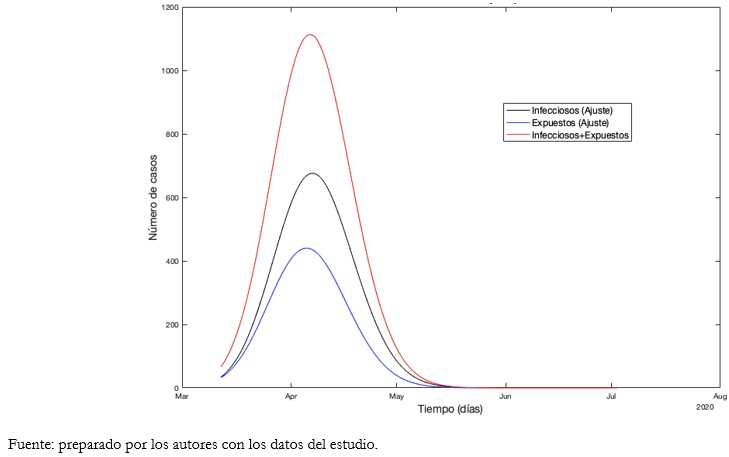
\includegraphics[width=\columnwidth]{Max personas expuestas escenario 3.jpg}
    \caption{Gráfico de máximo de personas expuestas e infectadas en el tercer escenario propuesto por Guerrero-Nancuante y colaboradores, elaborado por los mismos.}
    \label{grafico escenario 3}
\end{figure}

Tomando como ejemplo el trabajo hecho por Camilo Guerrero-Nancuante y Ronald Manríquez P, en su documento "Proyección epidemiológica de COVID-19 en Chile basado en el modelo SEIR generalizado y el concepto de recuperado"\cite{guerrero-nancuante_manriquezp_2020}, vemos un total de 3 escenarios de ejemplo que han dispuesto para su análisis.

\begin{enumerate}
    \item Aplicando los datos oficiales entregados por el Ministerio de Salud, con uso de numero de recuperados totales con el criterio establecido por ellos (14 días después de dar positivo).
    \item Aplicando datos oficiales, con protocolo de recuperación de 28 días, valor propuesto por la OMS y el Centro Europeo para la Prevención y Control de Enfermedades.
    \item Idéntico al segundo punto, salvo que se excluye a los fallecidos del total de recuperados (a diferencia de como lo hizo el MinSal en un inicio).
\end{enumerate}

Guerrero-Nancuante y colaboradores utilizaron un modelo SEIR idéntico al propuesto por Peng, que se explicó anteriormente. Para el tercer escenario, a mi parecer, el mejor para el estudio del COVID, los autores pronostican un total de 11 mil infectados acumulados hasta el 10 de agosto de 2020, una estabilización de la curva de infectados el 1 de mayo, y una cantidad mayor de recuperados en relación a infectados activos a partir de el 3 de septiembre, con un total de fallecimientos a fecha del 31 de agosto de 1151 personas.

Según los datos oficiales, sin embargo, a la fecha de 3 de septiembre de 2020, el total de personas fallecidas superaba los 15 mil, con un total de 375.044 casos activos confirmados a la fecha del 10 de agosto de 2020.

¿Qué fue lo que ocurrió? En general, la tendencia que se percibe al analizar los resultados de este tipo de predicciones, es que parecen ser muy poco acertadas. Sin embargo, en contexto de predicción a corto plazo, tal y como se analizó con el trabajo de Sánchez-Villegas y colaboradores, la simulación no siempre suele ser incorrecta. Para este caso en particular, puede ser que el modelo no haya sido el indicado, pues si bien para Peng y colaboradores si parece haber resultado correcto, el contexto en que se utilizó fue la sociedad China, que es tanto totalmente industrializada y capaz de proveer para sus ciudadanos, como socialista en naturaleza, reflejado en su enfoque de mantener la más mínima cantidad de casos y fallecidos como sea posible. Esto es imposible en el contexto Chileno, pues la capacidad del estado chileno para poder mantener periodos de cuarentena absolutos tal que china es nula.

¿Significa entonces que el uso de modelos es inutil, pues sus predicciones no son certeras? Para nada. Tal y como se dijo en un inicio, el uso de los modelos de predicción es tan solo tan bueno como el modelo mismo. Un modelo que no pueda reflejar las dinámicas sociales chilenas no puede ser empleado para predecir confiablemente el comportamiento del virus a tan largo plazo. Y pese a que es cierto de que eventualmente todos los modelos fallaron con la entrada de nuevas variantes, esto es solo producto de la falta de la inclusión del aparecimiento de variantes y reactivación de infecciones en los modelos. En retrospectiva parece algo obvio, pero era imposible de saber que el virus SarS-CoV-2 iba a tender a mutaciones tan extremas como las presentadas últimamente, sobretodo la variante Omicrón.
